\documentclass[11pt,a4paper]{report} 

% Für doppelseitigen Ausdruck (nur bei > 60 Seiten sinnvoll)
% \usepackage{ifthen}
% \setboolean{@twoside}{true}
% \setboolean{@openright}{true} 

% Deutsch
\usepackage[german]{babel} % deutsch und deutsche Rechtschreibung
\usepackage[utf8]{inputenc} % Unicode Text 
\usepackage[T1]{fontenc} % Umlaute und deutsches Trennen
\usepackage{textcomp} % Euro
\usepackage[hyphens]{url}
% statt immer Ab\-schluss\-ar\-beit zu schreiben
% einfach hier sammeln mit -. 
\hyphenation{Ab-schluss-ar-beit}
% Vorsicht bei Umlauten und Bindestrichen
\hyphenation{Ver-st\"ar-ker-aus-gang}
 % eigene Hyphenations, die für das Dokument gelten
\usepackage{amssymb} % Symbole
\usepackage{emptypage} % Wirklich leer bei leeren Seiten

%% Fonts, je ein kompletter Satz an Optionen

% Times New Roman, gewohnter Font, ok tt und serifenlos
%\usepackage{mathptmx} 
%\usepackage[scaled=.95]{helvet}
%\usepackage{courier}

% Palatino mit guten Fonts für tt und serifenlos
\usepackage{mathpazo} % Palatino, mal was anderes
\usepackage[scaled=.95]{helvet}
\usepackage{courier}

% New Century Schoolbook sieht auch nett aus (macht auch tt und serifenlos)
%\usepackage{newcent}

% Oder default serifenlos mit Helvetica 
% ich kann es nicht mehr sehen ...
%\renewcommand{\familydefault}{\sfdefault}

% ein bisschen eine bessere Verteilung der Buchstaben...
\usepackage{microtype}

% Bilder und Listings
\usepackage{graphicx} % wir wollen Bilder einfügen
\usepackage{subfig} % Teilbilder
\usepackage{wrapfig} % vielleicht doch besser vermeiden
\usepackage{listings} % schöne Quellcode-Listings
% ein paar Einstellungen für akzeptable Listings
\lstset{basicstyle=\ttfamily, columns=[l]flexible, mathescape=true, showstringspaces=false, numbers=left, numberstyle=\tiny}
\lstset{language=python} % und nur schöne Programmiersprachen ;-)
% und eine eigene Umgebung für Listings
\usepackage{float}
\newfloat{listing}{htbp}{scl}[chapter]
\floatname{listing}{Listing}

% Seitenlayout
\usepackage[paper=a4paper,width=14.2cm,left=36mm,height=22cm]{geometry}
\usepackage{setspace}
\linespread{1.15}
\setlength{\parskip}{0.5em}
\setlength{\parindent}{0em} % im Deutschen Einrückung nicht üblich, leider

% Seitenmarkierungen 
\newcommand{\phv}{\fontfamily{phv}\fontseries{m}\fontsize{9}{11}\selectfont}
\usepackage{fancyhdr} % Schickere Header und Footer
\pagestyle{fancy}
\renewcommand{\chaptermark}[1]{\markboth{#1}{}}
%\fancyhead[L]{\phv \leftmark}
\fancyhead[RE,LO]{\phv \nouppercase{\leftmark}}
\fancyhead[LE,RO]{\phv \thepage}
% Unten besser auf alles Verzichten
%\fancyfoot[L]{\textsf{\small \kurztitel}}
\fancyfoot[C]{\ } % keine Seitenzahl unten
%\fancyfoot[R]{\textsf{\small Technische Informatik}}

% Theorem-Umgebungen
\newtheorem{definition}{Definition}[chapter]
\newtheorem{satz}{Satz}[chapter]
\newtheorem{lemma}[satz]{Lemma} % gleicher Zähler wie Satz
\newtheorem{theorem}{Theorem}[chapter]
\newenvironment{beweis}[1][Beweis]{\begin{trivlist}
\item[\hskip \labelsep {\textit{#1 }}]}{\end{trivlist}}
\newcommand{\qed}{\hfill \ensuremath{\square}}

% Quellen teilen
\usepackage{bibtopic} 

% Hochschule Logo, noch nicht perfekt
\usepackage{hsmalogo}

% Spezialpakete
\usepackage{epigraph}
\setlength{\epigraphrule}{0pt} % kein Trennstrich

% damit wir nicht so viel tippen müssen, nur für Demo 
\usepackage{blindtext} 

% Zum Zeigen von Fehlern
\usepackage{soul}
\newcommand*\falsch{\st}

\usepackage{hyperref}
\hypersetup{
    colorlinks=true,
    linkcolor=blue,
    filecolor=magenta,      
    urlcolor=cyan,
    pdftitle={Overleaf Example},
    pdfpagemode=FullScreen,
    }

\newcommand{\tabitem}{~~\llap{\textbullet}~~}

\usepackage{xcolor}
\lstdefinestyle{customcs}{
  keywordstyle=\color{teal},
  identifierstyle=\color{violet},
  stringstyle=\color{orange}
}
 % alle Pakete und Einstellungen

% Hier anpassen 
\newcommand{\welchethesis}{Bachelor}
% \newcommand{\welchethesis}{Master}
\newcommand{\thesisofwas}{of Science}
\newcommand{\studiengang}{Technische Informatik}
% \newcommand{\studiengang}{Medizintechnik}
\newcommand{\titel}{Entwicklung eines Frameworks zur Darstellung von 
Smartphone-Sensordaten 
für die didaktische Unterstützung von Programmiervorlesungen}
\newcommand{\kurztitel}{Template Abschlussarbeit}
\newcommand{\autor}{Marius Cerwenetz}
\newcommand{\datum}{XX. Juli 2022} % Abgabedatum
\newcommand{\ort}{Mannheim}
\newcommand{\referent}{Prof.\ Dr.\ Peter Barth}
\newcommand{\korreferent}{Prof.\ Dr.\ Jens-Matthias Bohli}

\begin{document}
\begin{titlepage}
  % Kopf der Seite
  \hsmalogo[1] \hfill
  \parbox[b]{60mm}{
    % \textsf würde das Aussehen der ersten Seite ruinieren, 
    % wer will, soll das selbst außen rum machen...
    Fakultät Informationstechnik\\
    Studiengang \studiengang}
  \begin{center}
    % rumfiddeln, damit es für 4 Zeilen gerade noch so geht...
    \rule{1\textwidth}{1pt}\\[-3mm]
    \parbox[t][64mm]{110mm}{% 11 cm für Breite 13, ca. 7 für Höhe 6
      \begin{center}
        \Large{\welchethesis arbeit}\\[2mm]
        {\begin{spacing}{1.13} \huge \bfseries \titel \end{spacing}}
        \vfill
        \Large{\autor} \\[1mm] % keep space to window
        \ 
      \end{center}
    }
    \rule{\textwidth}{1pt}    
    \vfill    
    {\Large Abschlussarbeit} \\[5mm]
    {\large zur Erlangung des akademischen Grades} \\[5mm]
    {\large \welchethesis\ \thesisofwas} \\[5mm]
    \vfill    
    \begin{tabular}{ll} % Mitte der Seite
      Vorgelegt von & \autor \\
      am & \datum \\
      Referent & \referent \\
      Korreferent & \korreferent
    \end{tabular}    
    \vfill
  \end{center}
\end{titlepage}
\cleardoublepage


% Erklärung gemäß der Prüfungsordnung
\thispagestyle{empty}
\subsection*{Schriftliche Versicherung laut Studien- und Prüfungsordnung}

Hiermit erkläre ich, dass ich die vorliegende Arbeit selbstständig verfasst
und keine anderen als die angegebenen Quellen und Hilfsmittel benutzt habe.

\vspace{6em}
\noindent\begin{tabular}{p{0.37\textwidth}p{0.56\textwidth}}
\ort, \datum  & \rule{0.56\textwidth}{0.5pt}\\
              & \makebox[1cm]{\ } \autor
\end{tabular}

\vfill

\cleardoublepage

 % Titelseite, Erklärungen, etc.

\begin{abstract}
  Programmierenlernen fällt besonders am Anfang schwer.
  Embeddedprojekte erlauben mit vergleichsweise wenig Aufwand einen gelungen Einstieg mit effektiver Lernerfahrung.
  Solche Projekte benötigen allerdings viel Peripherie und Hardware.
  Diese benötigt wiederrum eine nicht niedrigschwellige Erfahrung zum Beispiel im Umgang mit Microcontrollern.
  Smartphones haben diese Nachteile nicht bieten allerdings trotzdem einen hohen Umfang an Sensoren.
  \\
  In dieser Arbeit wird ein Framework erstellt, dass das Smartphone nutzt um mit dem Microcontroller kleine Softwareprojekte umzusetzen.
  Kleine Aufgabenstellungen mit Musterlösungen werden ausgearbeitet und mitgereicht.
\end{abstract}

\tableofcontents

\chapter{Einführung} \label{chap:intro}
MINT-Berufe leiden hierzulande unter einem akuten Fachkräftemangel.
Das Institut der deutschen Wirtschaft ermittelte für April 2021 ein Unterangebot von 145.100 Personen \cite{mint_jahresreport} in 36 MINT-Berufskategorien. 
Digitalisierungs-Projekte geraten dadurch ins Stocken.
\\
Nicht zuletzt er auch ein Kräftemangel in der Softwareentwicklung.
Es fehlen Programmiererinnen und Programmierer.
Softwareentwicklung ist gerade in der Lernphase nicht trivial und abstrakt.
Unlebendige Übungsaufgaben die beispielsweise Konsolenein- und ausgaben realisieren schrecken zukünftige Programmierinnen und Programmierer eher ab als sie zu ermutigen.
\\
Microcontroller sind bereits eine große Hilfe, da hier spielerisch kleine Projekte realisiert werden können.
So können schon früh in Schulen Kinder an die Programmierung herangerführt werden.
Sie lernen spielerisch kleine Programme zu entwickleln und verstehen die ihnen beigebrachten Abläufe durch schnelle Anwendung.
Microcontroller sind jedoch auch mit Anschaffungskosten verbunden und für kleine Anwendungen, welche Sensoren verwenden, wird viel zusätzliches Material wie zum Beispiel Breadboards, Verbindungskabel und Erweiterungsboards benötigt.
Moderne Smartphones bieten hier Abhilfe da Sie meistens mit verschiedenen Sensoren bespickt sind, wie zum Beispiel: Kompass, GPS, Microphon oder Kamera.
Viele Kinder besitzen bereits mit 10 Jahren \cite{bitkom_smartphones} ein Smartphone. 
\\
Im Rahmen dieser Arbeit soll ein Framework entwickelt werden, dass das Smartphone von Anwendern einbindet um Sie beim Programmierenlernen zu unterstützen.
Dies soll in Form von Aktivitäten möglich sein. Aktivitäten starten entweder UIs auf dem Smartphone um eine Eingabe entgegenzunehmen oder senden konstant Sensordaten.

\chapter{Experimente/Aufgaben} \label{chap:Experimente}

\section*{Aufgaben}
Dieses Kapitel enthält verschiedene Beispielaufgaben die mit dem Framework gelöst werden sollen.
Die Benutzung der API dazu wird später geschildert.


\textbf{Disco}\\
Die LED muss ganz schnell blinken.
Ablauf: \verb|led_on, sleep, led_off ...|
\\

\textbf{Diebstahl-Alarm}\\
Wenn nach dem Telefon gegriffen wird soll die LED blinken.
Wenn man sich davon entfernt soll sie wieder aus sein.
\\

\textbf{Würfeln}\\
Das Smartphone wird geschüttelt.
Ein random Zahlenwert wird zurückgegeben.
Je nachdem welches Ergebnis zurückkommt soll ein Wert auf dem Display angezeigt werden.

Ablauf: \verb|get_random(), displayText|

\textbf{Klatsch-Zähler}\\
Der Anwender möchte wissen wie oft in einem bestimmten Zeitraum geklatscht wurde.
Ein Methodenaufruf startet in der Androidanwendung eine Activity, die innerhalb des im Argument genannten Zeitraums die Anzahl der maximalen Lautstärkeamplituden des Mikrophons misst und die Anzahl zurückgibt.
\begin{figure}[htbp]
  \centering
  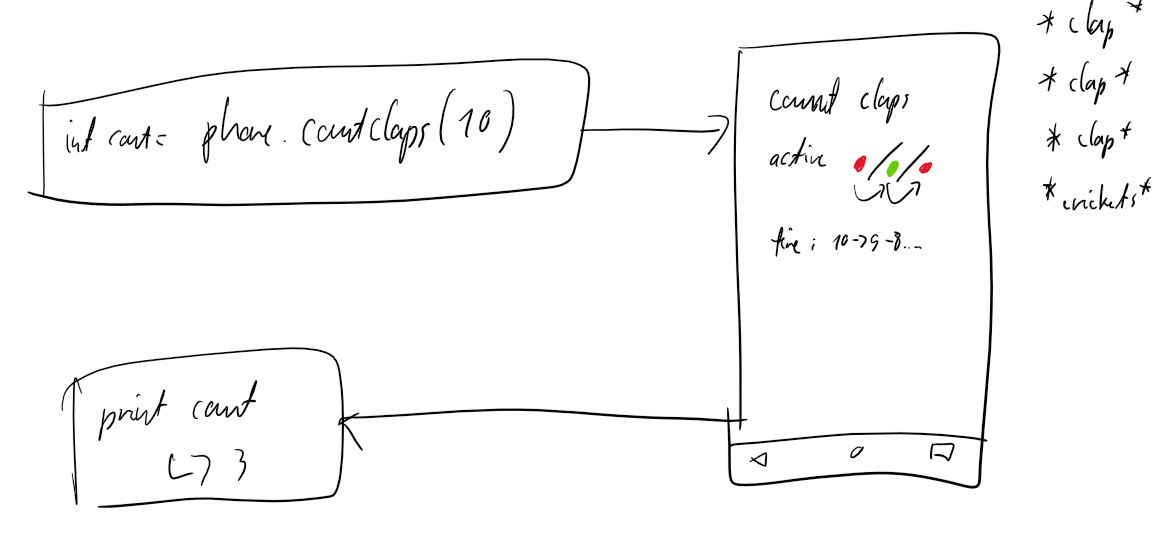
\includegraphics[width=.9\textwidth]{images/count_claps.png}
  \caption{Klatsch-Zähler}
  \label{fig:clap_count}
\end{figure}

\textbf{Dreh-Zähler}\\
Ein Nutzer möchte in einem bestimmten Zeitraum zählen wie oft das Smartphone gedreht wurde.



\section*{API}
Gelöst werden sollen die Aufgaben durch das Aufrufen der API.
Diese bietet die benötigten Funktionen an.
Die Aufrufe sind frei miteinander kombinierbar, so dass Aufgaben erweitert werden können.

\subsection*{Eingaben}

\textbf{Auslesen der accelerometer-Daten}\\
Ein User will den Wert der X, Y und Z Koordinaten des Smartphones wissen.
So kann er bspw. feststellen, ob das Smartphone gerade nach unten, oben oder horizontal bewegt wurde.
Kippbewegungen werden nicht detektiert.
\lstinputlisting[]{listings/api/acc.c}

\textbf{Lautstärkepegelmessung}\\
Ein User möchte den aktuellen Lautstärkepegel messen.
\lstinputlisting{listings/api/vol.c}

\textbf{Annäherungssensor-Messung}\\
Ein User möchte wissen, ob ein Objekt unmittelbar vor den Annäherungssensor steht.
Der Aufruf erfolgt folgendermaßen.
\lstinputlisting{listings/api/proxy.c}

\subsection*{Ausgaben}

\textbf{Display-Ausgabe}\\
Um auf dem Smartphone einen beliebigen Text anzuzeigen.
Dies kann er zum Beispiel wie im folgenden Beispielcode machen.
\lstinputlisting[]{listings/api/display.c}

\textbf{LED leuchten lassen}\\
Ein User möchte eine "LED" auf dem Display ansteuern.
Dies kann er so machen.
\lstinputlisting[]{listings/api/led.c}

\textbf{Vibrationsauslöser}\\
Ein Nutzer möchte das Smartphone auf Anfrage virbrieren lassen.
Der Aufruf einer Methode lässt das Smartphone einmal vibrieren.
\lstinputlisting[]{listings/api/vib.c}

\textbf{Audio-Ausgabe}\\
Ein Nutzer möchte den Pfad zu einer Audio-Datei angeben und
\lstinputlisting[]{listings/api/vib.c}




\chapter{Einführung} \label{chap:einfuehrung}
% Das Smartphone soll für das Austauschen von Daten verwendet werden.
% Hier wird klar unterschieden in Anfragen die eine Benutzerinteraktion verlangen und welche, die passiv Daten auslesen.
% Die Übertragung wird nach dem Request-Response-Prizip realisiert.
% Das Framework besteht aus drei großen Teilen:
% \begin{enumerate}
%   \item Einer Anwendung auf einem Android-Smartphone
%   \item Einer Middleware auf dem PC oder Laptop des Anwenders
%   \item Einer Bibliothek in Java, C++ und Python ebenfalls auf PC oder Laptops des Anwenders
% \end{enumerate}
% \begin{figure}[htbp]
%   \centering
%   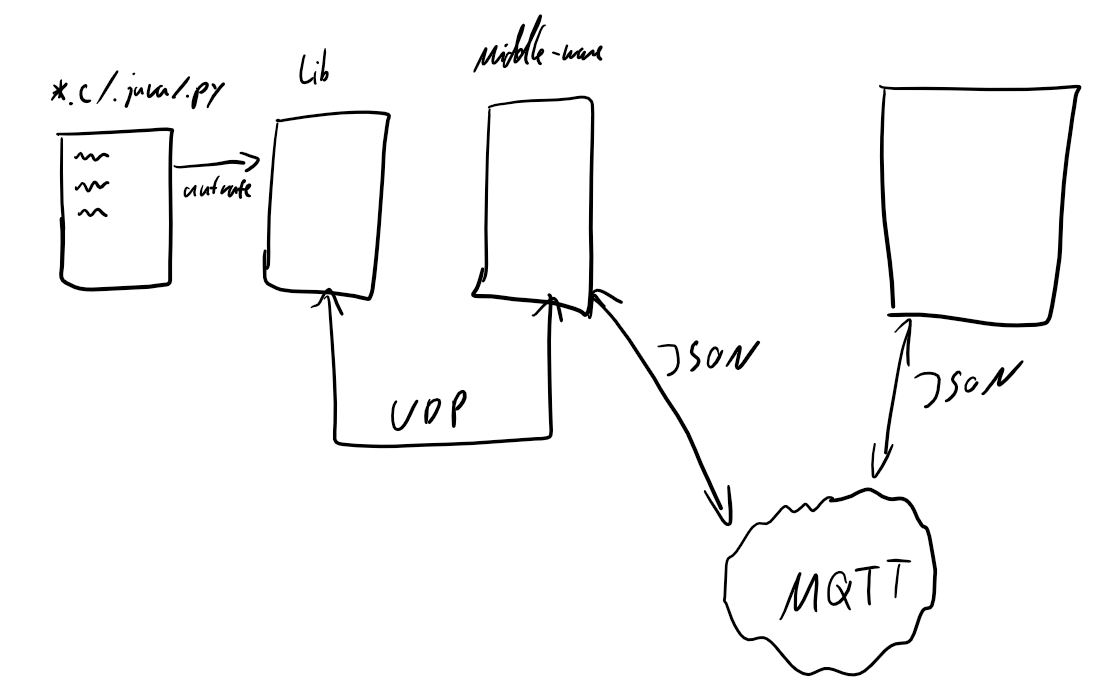
\includegraphics[width=.9\textwidth]{images/design.png}
%   \caption{Framework-Ablauf}
%   \label{fig:Ablauf}
% \end{figure}
% Auf die Funktionsweise und den Ablauf wird im folgenden genauer eingegangen.

% \section*{Bibliothek und API}
% Zur Ansteuerung des Smartphones werden vier Softwarebibliotheken jeweils in den Programmiersprachen Python, C++, C und Java zur Anbindung realisiert.
% Die Bibliotheken in den den Programmiersprachen C++, Java und Python dienen zur Erstellung von Smartphone-Objekten über die Methodenaufrufe realisiert werden können.
% Die Bibliothek in C ist prozedural realisiert und bietet den Aufruf von globalen Methoden ohne Objektbindung.
% \\
% Die Afrufe sind logisch in zwei Kategorien geordnet: Dem Aufruf zur Übermittlung von Sensordaten und dem Aufruf zum Starten von Activites zwecks einer Nutzerbedienung mit anschließendem Rückübermitteln der Nutzerauswahl.
% \\
% Die Anfragen werden in der jeweiligen Programmiersprache angestoßen und werden im weiteren Verlauf von der Middleware über das UDP-Protokoll auf dem gleichen PC entgegengenommen.
% \section*{Middleware}
% Die Middleware dient als Vermittlungsschicht zweichen Bibliothek und Smartphone.
% Sie nimmt per UDP Methodenaufrufe entgegen und sendet diese als Nachricht für das Smartphone weiter.
% Die Nachricht wird dabei über einen MQTT-Server übertragen.

% \subsection*{MQTT}
% Die Nachrichten werden von der Middleware per MQTT übertragen.
% MQTT beziehungsweise Message Queuing Telemetry Transport, ist ein Netzwerkprotokoll.
% Es dient der Übertragung von Messdaten.
% Sensor-Geräte senden dabei Nachrichten an einen Broker in ein Topic.
% Ein Broker ist eine MQTT-Serverkomponente die Nachrichten annimt.
% Broker verwalten die gesendeten Daten hierarchisch in Themenberereichen, den Topics.
% Andere Geräte können am Broker Topics abbonieren (subscribe).
% Publiziert nun der Sensor-Client einen neuen Messwert auf einem Topic das ein Empfänger abboniert hat wird ihm die Nachricht zugestellt.
% \\
% Die Nachrichten werden dabei mit einem Quality of Service-Flag übertragen.
% Dies beschreibt die Sicherungsgarantie mit der eine Nachricht übermittelt wird.
% Sie ist aufgeteilt in drei Stufen
% \begin{enumerate}
%   \item at most once
%   \item at least once
%   \item exactly once
% \end{enumerate}
% In der ersten Stufe werden Nachrichten zwar übermittelt, jedoch kann es vorkommen, dass bei Verbindungsabbrüchen Nachrichten nicht weitergeleitet werden.
% \\
% In der zweiten Stufe werden Nachrichten so lange versendet, bis Clienten die das jeweilige Topic abboniert haben eine Empfangsbestätigung senden.
% Es wird jedoch nicht sichergestellt, ob die Nachricht nicht mehrmals versand wurde.
% \\
% Dies wird in der dritten Stufe, exactly once, sichergestellt. 
% Nachrichten werden nur so lange gesendet bis die Übertragung einmal bestätigt wurde.

\subsection*{Nachrichtenformate}
Die Nachrichten werden im JSON-Format übertragen.
Für die Anwendung steht folgender Ausschnitt beispielsweise für das Starten einer bestimmten Activity.
\begin{lstlisting}
  {
    "issue_id" : 0,
    "type" : activity_request,
    "value" : "boolean_activity",
    "arguments" : []
  }
\end{lstlisting}
Das Type-Feld beschreibt, ob es sich bei der Nachricht um ein request oder um eine response handelt.
Dieses Feld kann die folgenden Werte annehmen:
\begin{itemize}
  \item activity\_request
  \item activity\_response
\end{itemize}
Ein Activity-Request fordert das Starten einer Activity mit der der Nutzer interargieren muss.
Je nach Request-Art werden entweder Sensor-Responses oder Activity-Responses zurückgesendet.


\section*{Android Anwendung}
Die Android-Anwendung läuft auf dem Smartphone des Anwenders.
Sie hat ein sehr schlichtes äußeres Erscheinungsbild und reagiert nur auf Anfragen der Middleware.
Sie besteht aus einer Haupt-Activity und mehreren Unter-Activites die gegebenenfalls aufgerufen werden.
\\
In der Haupt-Activity wird ein Service gestartet und gebunden.
Der Service baut eine Verbindung zu einem MQTT Topic auf einem MQTT-Server auf, reagiert auf Nachrichten und versendet gegebenenfalls selbst Nachrichten.
Geht eine Nachricht ein die eine User-Interaktion verlangt wird die jeweilige Activity gestartet.
Der User interargiert mit der Activity und bestätigt seine Eingabe.
Die Activity bindet daraufhin den MQTT-Service und versendet die Antwort an die Middleware, wo Sie an die Bibliothek und somit an die Endanwendung auf dem PC des Users gesendet wird.
\\
Geht eine Nachricht ein, die die Übermittlung von Sensordaten verlangt wird keine eigene Aktivität gestartet.
Der Service startet in diesem Fall selbst den Ausleseprozess und übermittelt dann, je nach Anfrage, einen oder mehrere Werte.
Die Verfügbarkeit der jeweiligen Sensoren wird beim Start der Anwendung ermittelt.
Falls ein Sensor angefragt wird der auf dem Smartphone nicht existiert wird eine Nachricht mit einer Fehlermeldung zurückgegeben.
\begin{figure}[htbp]
  \centering
  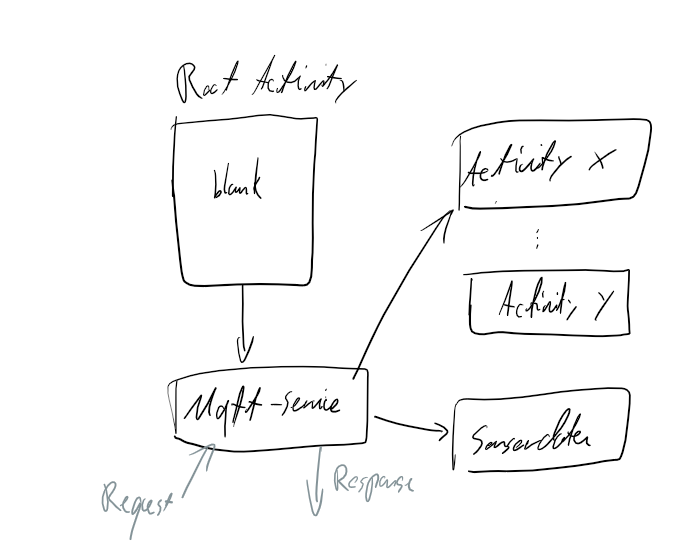
\includegraphics[width=.9\textwidth]{images/android_app.png}
  \caption{Android-App-Aufbau}
  \label{fig:android_app}
\end{figure}





\chapter{Diskussion und Fazit} \label{chap:fazit}
\chapter{Ausblick} \label{chap:fazit}

% Listen wenn überhaupt ans Ende und nicht an den Anfang.
% Meist ist das aber unnötig.
% \listoffigures % Liste der Abbildungen 
% \listoftables % Liste der Tabellen
% \newpage

\bibliographystyle{plain} % Literaturverzeichnis
\begin{btSect}{thesis} % mit bibtopic Quellen trennen
\addcontentsline{toc}{chapter}{Literaturverzeichnis und Online-Quellen}
\section*{Literaturverzeichnis}
\btPrintCited
\end{btSect}
\begin{btSect}{online}
\section*{Online-Quellen}
\btPrintCited
\end{btSect}
% dann mit "bibtex thesis1" und "bibtex thesis2" arbeiten

\end{document}
;;; Local Variables:
;;; ispell-local-dictionary: "de_DE-neu"
;;; End:
